% --- CONTENT FOR: Sections/4_Timeline.tex ---
\section{Provisional Timeline}

The group has established a provisional timeline (GANTT Chart) to track key deliverables. Figure \ref{fig:gantt} illustrates the high-level schedule. And was made using Notion App, as it is free and could fit our mork style for each of us.

\begin{figure}[H]
    \centering
    % Using Cranfield Logo as placeholder for GANTT Chart as requested
    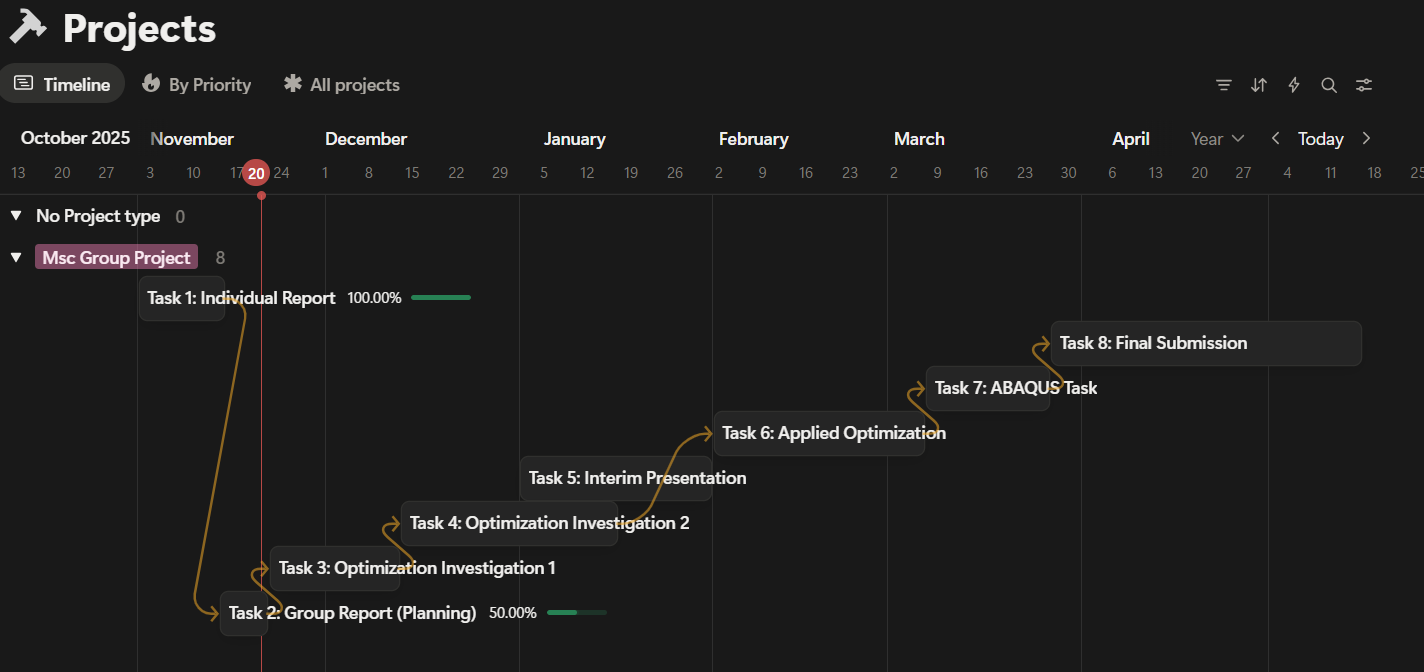
\includegraphics[width=0.8\textwidth]{Images/GANTT.png}
    \caption{Provisional GANTT Chart for Group Chenonceau, updated on 11/20/2025}
    \label{fig:gantt}
\end{figure}

The key milestones derived from the module brief \cite{phillips2025brief} are listed in Table \ref{tab:deadlines}.

\begin{table}[H]
\centering
\caption{Key Project Deadlines}
\label{tab:deadlines}
\begin{tabular}{l l l}
\toprule
\textbf{Task} & \textbf{Description} & \textbf{Deadline} \\
\midrule
Task 2 & Group Report (Planning) & 21/11/2025 \\
Task 3 & Optimisation Investigation 1 & 12/12/2025 \\
Task 4 & Optimisation Investigation 2 & 16/01/2026 \\
Task 5 & Interim Presentation & Jan 2026 \\
Task 6 & Applied Optimisation & 06/03/2026 \\
Task 7 & ABAQUS Task & 26/03/2026 \\
Final & Final Submission (Parts 1, 2, 3) & 15/05/2026 \\
\bottomrule
\end{tabular}
\end{table}